\section{Modelado de la información}
\subsubsection{Interesados identificados}
Por el ámbito de la herramienta se llegó a la conclusión que los interesados son todas las personas que puedan llegar a utilizar el Datapower como herramienta de trabajo, bien sean desarrolladores o administradores:
\begin{itemize}
    \item Administradores de Datapower
    \item Desarrolladores de Datapower
\end{itemize}
\begin{figure}[th!]
    \centering
    \includegraphics[width=1.0\textwidth]{DesarrolloInvestigacion/images/Interesados.png}
    \caption{Interesados Identificados}
\end{figure}
\subsubsection{Intereses}
Gracias a las entrevistas realizadas a los diferentes administradores, se pudo determinar un listado de los intereses que este grupo tiene respecto a su interacción con el Datapower:
\begin{itemize}
    \item Despliegues de configuración en cada Datapower
    \item Cargues de XML
    \item Manejo host alias
    \item Creación de backups
    \item Manejo de certificados
    \item Verificación de conectividad
    \item Configuración de:
    \begin{itemize}
        \item XML Firewalls
        \item Grupos de balanceo
        \item Multiprotocol gateway.
    \end{itemize}
    \item Manejo de métricas
    \item Revisión de logs en ambientes productivos.
    \item Dificultad en los monitoreo.
    \item Monitoreo de estado de objetos en los Datapower.
\end{itemize}
\subsubsection{Modelo conceptual de dominio}
Con el listado de intereses se define un modelo conceptual que permite facilitar el modelado de la información obtenida
\begin{figure}[th!]
    \centering
    \includegraphics[width=1.0\textwidth]{DesarrolloInvestigacion/images/Modelo_de_dominio.png}
    \caption{Interesados Identificados}
\end{figure}
\subsubsection{Activos de información}
Realizando un análisis a profundidad de las entrevistas realizadas, permite identificar activos de información para realizar un futuro análisis categórico y meta categórico.
\newline ver anexo activos de información
\subsubsection{Análisis de categorías}
Ya teniendo los activos de información, se determinan las categorías que enmarcan esos activos de información:
\begin{itemize}
    \item Ambientes: Desarrollo, Pruebas y Producción
    \item Rol
    \item Usuario
    \item Acciones
    \item Dominios
    \item Tipos de Datapower: Interno y Externo
    \item Grupo Datapower
    \item Grupo de Balanceo
    \item Objeto Configuración Datapower
    \item Log: Default, Performance, Rastreo, Errores, Access, Debug, Probe
    \item Valores a Monitorear
    \item Métodos Acceso Datapower (CLI, WebGUI, SOMA)
    \item Servicio Web
    \item Atributos Servicios (Fecha, Tamaño, Cliente, Código http)
    \item Backup (Normal, Seguro)
    \item Certificados Digitales (Privados, Públicos)
    \item Originador Certificado
    \item Tareas
\end{itemize}
\subsubsection{Descripción meta-categórica}
Con el análisis categórico de los diversos activos de la información obtenemos un modelo inicial de las principales meta categorías determinadas:
\begin{figure}[th!]
    \centering
    \includegraphics[width=1.0\textwidth]{DesarrolloInvestigacion/images/ModeloInicial.png}
    \caption{Modelo de información inicial}
\end{figure}
Ahora se hace el modelo de información, que evidencia las relaciones entre las meta categorías identificadas, este se obtuvo con la información levantada de las entrevistas y adicionalmente con la experiencia que tiene uno de los integrantes del equipo en el manejo de la plataforma Datapower.
\begin{figure}[th!]
    \centering
    \includegraphics[width=1.0\textwidth]{DesarrolloInvestigacion/images/ModeloMetaCategorias.png}
    \caption{Modelo de información}
\end{figure}
\subsubsection{Modelo entidad relación}
Ya con el modelo de información obtenido, se aterriza este en una versión inicial del modelo entidad relación que soportara el prototipo de la herramienta de administración centralizada para Datapower.
\begin{figure}[th!]
    \centering
    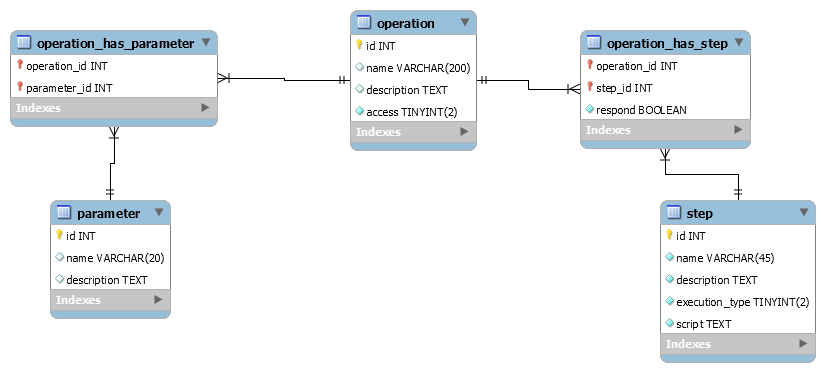
\includegraphics[width=1.0\textwidth]{DesarrolloInvestigacion/images/ModeloEntidadRelacion2.png}
    \caption{Modelo Entidad Relación del Motor}
\end{figure}
\begin{figure}[th!]
    \centering
    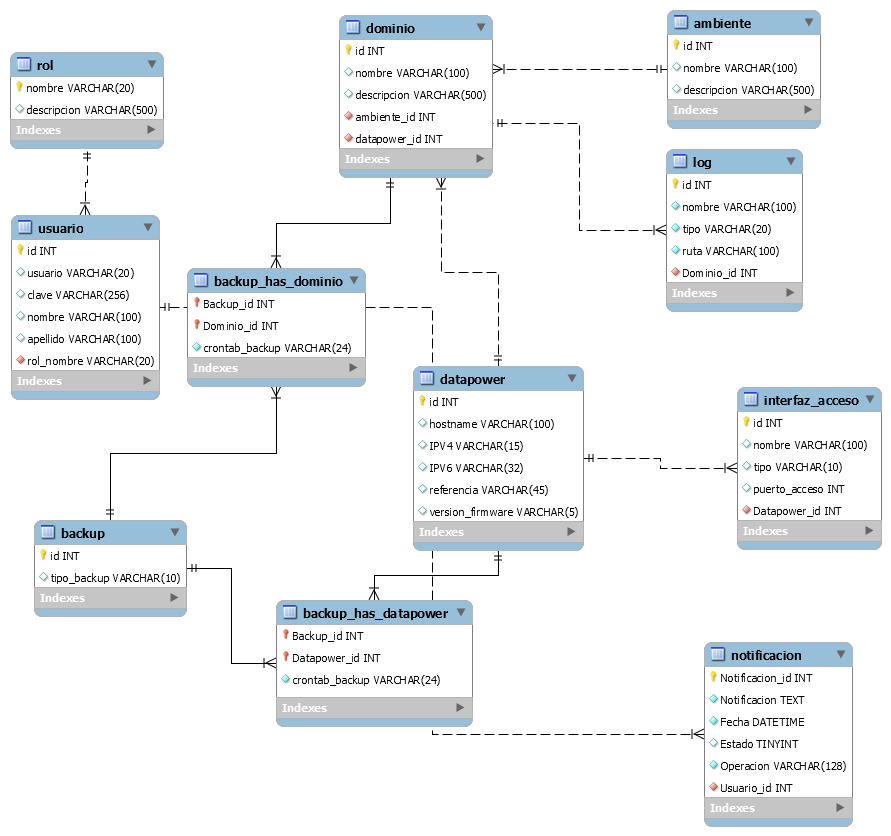
\includegraphics[width=1.0\textwidth]{DesarrolloInvestigacion/images/ModeloEntidadRelacion1.png}
    \caption{Modelo Entidad Relación de Administración}
\end{figure}
